\documentclass[a4paper, 12pt]{article}
\usepackage{listings} 
\usepackage{xcolor}
\usepackage{mdframed}
\usepackage{graphicx}
\usepackage{pgfplots}
\usepackage{float}
\usepackage{mathtools}
\usepackage[margin=1.00in]{geometry}
\DeclarePairedDelimiter\ceil{\lceil}{\rceil}
\DeclarePairedDelimiter\floor{\lfloor}{\rfloor}

\definecolor{code-gray}{gray}{0.93}
\begin{document}
\title{ECE 341 - Lab \#10}
\author{Collin Heist}
\date{\today}
\maketitle
\pagenumbering{roman}
\tableofcontents
\lstlistoflistings
\newpage
\pagenumbering{arabic}

\section{Introduction}
The purpose of this lab is to use the PIC32 to measure the frequency of events. For this particular lab, we'll be spinning a motor connected to the board and using outputs from hall effect sensors, as well as the input capture peripheral, to measure the rotational frequency of the motor. 

In this lab, we'll be using two 'new' peripherals. One is the output compare (PWM) peripheral we'll be using to power the motor at various speeds; and the second (actually new) peripheral is the input capture peripheral. This peripheral will trigger on a variable number of pulse edges on the input pin. This will be used so that when the hall effect sensors on the motor turn on / off, the rise or fall of that signal will trigger the input capture interrupt, allowing us to analyze the timing of the event.

\section{Implementation}
Just like all the other labs, the first and most important function is the system initialization. This is shown below in Listing  \ref{lst:sysinit}.

	\begin{mdframed}[backgroundcolor=code-gray, roundcorner=10pt,
								innerleftmargin=5, innertopmargin=5, innerbottommargin=5]	
	\begin{lstlisting}[language=C, caption=System Initialization, tabsize=2, label={lst:sysinit}]
	void system_init() {
		Cerebot_mx7cK_setup();
		PORTSetPinsDigitalOut(IOPORT_B, SM_LEDS);
		PORTSetPinsDigitalOut(IOPORT_D, BIT_1);
		LATBCLR = SM_LEDS;
		LATDCLR = BIT_1; 

		init_LCD();
		reset_clear_LCD();

		PORTSetPinsDigitalIn(IOPORT_D, BIT_3 | BIT_12);
		mIC5ClearIntFlag();	
		OpenCapture5(IC_ON | IC_CAP_16BIT | IC_IDLE_STOP |
			IC_FEDGE_FALL | IC_TIMER3_SRC |
			IC_INT_1CAPTURE | IC_EVERY_FALL_EDGE);
		ConfigIntCapture(IC_INT_ON | IC_INT_PRIOR_3 |
			IC_INT_SUB_PRIOR_0);
	
		mCNOpen(CN_ON, (CN8_ENABLE | CN9_ENABLE), 0);
		mCNSetIntPriority(1);
		mCNSetIntSubPriority(0);
		unsigned int x = PORTReadBits(IOPORT_G, BTN1 | BTN2);
		mCNClearIntFlag();
		mCNIntEnable(1);

		OpenTimer3(T3_ON | T3_SOURCE_INT | T3_PS_1_256, 0xFFFF);
		mT3SetIntPriority(2);
		mT3SetIntSubPriority(2);
		mT3IntEnable(1);

		init_pwm(40, 1000);

		INTEnableSystemMultiVectoredInt();
	}
	\end{lstlisting}
	\end{mdframed}
	
Once again, I will be using the LCD to output the current status of the speed readings, as well as the PWM output based off the button status'. The next section of code initializes the input capture module. Bit 3 and 12 are the two tachometer inputs (even though we'll only be using one). For this program, I'll be using input capture \#5, with an associated 16-bit timer that triggers on falling edges, is tied to timer 3, and has no prescale counter. Like previous labs, the change notice peripheral is also configured for buttons 1 and 2 so that I can change the PWM output in real-time. Timer 3 is used with the input capture peripheral, and is set to the highest possible value in the period register, with a prescale value of 256. I will not show the timer 3 interrupt routine, but it simply toggled \textbf{LEDC} and clears the interrupt flag. Finally, the PWM is initialized for a 40\% duty cycle and 1,000 Hz frequency.

The specific setup for the input capture is quite complicated but very important. We use a 16-bit timer because timer 3 is only 16-bits, it triggers on falling edge but this is structurally equivalent to triggering on rising edges (just with a phase shift for the first reading). The peripheral can be configured to trigger the interrupt on 1, 2, 4, or 16 of these edges and for purposes of this lab it is triggered every edge. The interrupt is given a priority level of three so that when the motor completes a rotation, this timing evaluation happens immediately. This might have additional consequences because the ISR for this peripheral is quite long compared to the others, meaning some timing interrupts could be less accurate in this current scheme.

Button presses in this program are structurally the same as the previous lab. Each different button combination corresponds to a different duty cycle for the motor. The only difference is that this lab just uses the top line of the LCD to display the current duty cycle. That code is shown below in Listing \ref{lst:cnisr}.

	\begin{mdframed}[backgroundcolor=code-gray, roundcorner=10pt,
								innerleftmargin=5, innertopmargin=5, innerbottommargin=5]	
	\begin{lstlisting}[language=C, caption=Change Notice ISR, tabsize=2, label={lst:cnisr}]
	void __ISR(_CHANGE_NOTICE_VECTOR, IPL1) CNIntHandler(void) {
		LATBINV = LEDB;
		hw_ms_delay(20);
		unsigned int buttons = read_buttons();
		unsigned int pwm_cycle = decode_buttons(buttons);
		set_pwm(pwm_cycle);

		char pwm_str[8] = {'\0'};
		sprintf(pwm_str, "%u\%", pwm_cycle);
	
		char lcd_str[50] = "PWM Cycle: ";
		strcat(lcd_str, pwm_str);

		set_cursor_LCD(FIRST_LINE_START);
		put_string_LCD("				");
		set_cursor_LCD(FIRST_LINE_START);
		put_string_LCD(lcd_str);

		LATBINV = LEDB;
		mCNClearIntFlag();
	}
	\end{lstlisting}
	\end{mdframed}
	
After reading the buttons and obtaining the corresponding duty cycle, a string is generated with the updated value. Since the LCD is shared between the background and foreground tasks, I ensure the location of the cursor on the LCD is correct by setting it to the beginning of the first line, clearing that line by writing 16 spaces (as the LCD is 16 characters wide), resetting the location and \textit{finally} writing the formatted string to the LCD. \textbf{LEDB} is then toggled at the end of the interrupt for debugging / monitoring purposes, just before the interrupt flag is cleared.

The newest foreground task is the input capture module. This interrupt routine is triggered when the motor sensor's are triggered on / off. Therefore, this following code (Listing \ref{lst:icisr}) is what actually performs the speed calculation:

	\begin{mdframed}[backgroundcolor=code-gray, roundcorner=10pt,
								innerleftmargin=5, innertopmargin=5, innerbottommargin=5]	
	\begin{lstlisting}[language=C, caption=Input Capture ISR, tabsize=2, label={lst:icisr}]
	void __ISR(_INPUT_CAPTURE_5_VECTOR, IPL3) IC5Handler (void) {
		LATBINV = LEDD;
		unsigned int input_buffer[4] = {0};
		static unsigned short int new_capture = 0;
		static unsigned short int old_capture = 0;
		unsigned short int delta_t = 0;

		ReadCapture5(input_buffer);
		new_capture = input_buffer[0];
		delta_t = new_capture - old_capture;
		old_capture = new_capture;

		float rev_per_sec = 10.0E6 / 256.0 / (float) delta_t;
		unsigned int i = 0;
		for (i = BUFFER_LEN-1; i > 0; i--)
			rps_buffer[i] = rps_buffer[i-1];
		rps_buffer[0] = rev_per_sec;

		mIC5ClearIntFlag();
	}
	\end{lstlisting}
	\end{mdframed}
	
The variable \textbf{input\_buffer} is an array of unsigned integers, despite us only caring about a single variable from the timer on the input capture module. This is because there can be at most four values read from the input capture peripheral at once, and so an entire buffer needs to be passed in at once. The variables for the new and old capture times are \textbf{static} because their values need to persist between instances of the interrupt triggering. Because the time difference between the tachometer outputs correspond to a full rotation of the motor, two triggers of the interrupt are required to obtain a reasonable reading for the RPS.

\textbf{ReadCapture5()} fills the buffer with the value of the timer at the time of the interrupt trigger. That value is stored as the new capture time, and the corresponding $\delta t$ is then calculated. This equates to how long between a full rotation of the motor. The next section of code converts that raw difference in the timer register to the current revolutions per second, and then stores that inside the buffer at position 0. To keep this buffer changing in order to calculate a rolling average, all values of the buffer are shifted down an element before this addition occurs. This buffer is declared as a global variable (with values of zero) and a length defined in the header file, which I used 32 values for this particular lab.

The calculation for the RPS from a given timer count difference is shown below:

$$RPS=\frac{f_{PB}}{t_{ps}}\cdot \frac{1}{t_{diff}}$$

The code in Listing \ref{lst:icisr} exactly matches this above function, with the only difference being I used pre-defined values for $f_{pb}$ and $t_{ps}$, as they are constant throughout the program's operation.

With all of these functions written, the \textbf{main()} function is implemented as follows:

	\begin{mdframed}[backgroundcolor=code-gray, roundcorner=10pt,
								innerleftmargin=5, innertopmargin=5, innerbottommargin=5]	
	\begin{lstlisting}[language=C, caption=Main Program Loop, tabsize=2, label={lst:main}]
	int main() {
		system_init();

		while (1) {
			hw_ms_delay(100);
			mCNIntEnable(FALSE);
		
			float avg = 0;
			unsigned int i = 0;
			for (i = 0; i < BUFFER_LEN; i++)
				avg += rps_buffer[i];
			avg /= BUFFER_LEN;

			char lcd_str[16] = {'\0'};
			sprintf(lcd_str, "Average: %06.2f", avg);
			set_cursor_LCD(SECOND_LINE_START);
			put_string_LCD("				");
			set_cursor_LCD(SECOND_LINE_START);
			put_string_LCD(lcd_str);
	
			mCNIntEnable(TRUE);
		}

		return 1;
	}
	\end{lstlisting}
	\end{mdframed}
	
Every one hundred milliseconds, the change notice interrupts are disabled (to prevent interference with the LCD), the current average value of the previous \textbf{BUFFER\_LEN} values in the RPS buffer are calculated. A string is then constructed that displays the average RPS value inside this buffer. This is placed on the second line of the LCD (in a similar way as the previous duty cycle).

Obviously the way I calculated the moving average is a bit slow for larger RPS buffers, as the entire buffer is iterated over each loop of \textit{main}; however this is a very simple and easy to implement average for the purposes of this lab. I chose to use a rolling buffer (whose values are shifted down each time a new value is added) because this is also very easy to implement, and does not deal with any pointer logic, or modulating around the buffer's length with index values.

\section{Testing and Verification}
Testing for this lab was very straightforward. Each separate task utilizes a different LED (such as D in the input capture ISR, etc.), so hooking each of these probes onto the oscilloscope verified all of these values at the same time. The captures for the four button combinations are shown in Figures \ref{fig:duty40}, \ref{fig:duty65}, \ref{fig:duty80}, and \ref{fig:duty95}. In all of the following captures: $D_0$ is \textbf{LEDA} (the timer 2 ISR), $D_1$ is \textbf{LEDB} (the change notice ISR), $D_2$ is \textbf{LEDC} (the timer 3 ISR), and $D_3$ is \textbf{LEDD} (the input capture ISR).

\begin{figure}[H]
\centering
\includegraphics[width=.8\textwidth]{scope_0.png}
\caption{40\% Duty Cycle}
\label{fig:duty40}
\end{figure}

\begin{figure}[H]
\centering
\includegraphics[width=.8\textwidth]{scope_1.png}
\caption{65\% Duty Cycle}
\label{fig:duty65}
\end{figure}

\begin{figure}[H]
\centering
\includegraphics[width=.8\textwidth]{scope_2.png}
\caption{80\% Duty Cycle}
\label{fig:duty80}
\end{figure}

\begin{figure}[H]
\centering
\includegraphics[width=.8\textwidth]{scope_3.png}
\caption{95\% Duty Cycle}
\label{fig:duty95}
\end{figure}

\begin{table}[ht]
\centering
\begin{tabular}{c|c|c|c}
\textbf{Duty Cycle (\%)} & \textbf{$V_M$ (V)} & \textbf{$f_{SB}$ (Hz)} & \textbf{Speed (RPS)} \\
\hline
0 & 7.915 & 0 & 0 \\
40 & 7.895 & 307 & 305.85 \\
65 & 7.890 & 417 & 435.05 \\
80 & 7.884 & 483 & 467.6 \\
95 & 7.882 & 485 & 491.32 \\
\end{tabular}
\end{table}

The captures of all of this data are shown in Figures \ref{fig:data0}, \ref{fig:data40}, \ref{fig:data65}, \ref{fig:data80}, and  \ref{fig:data95} at the end of the report.

The supply voltage clearly drops as the duty cycle increases, and this is a result of the increased \textit{load} on the power supply. Due to the increasing current draw from the motor, the power supply is unable to maintain the desired potential difference across the terminals.

\begin{center}
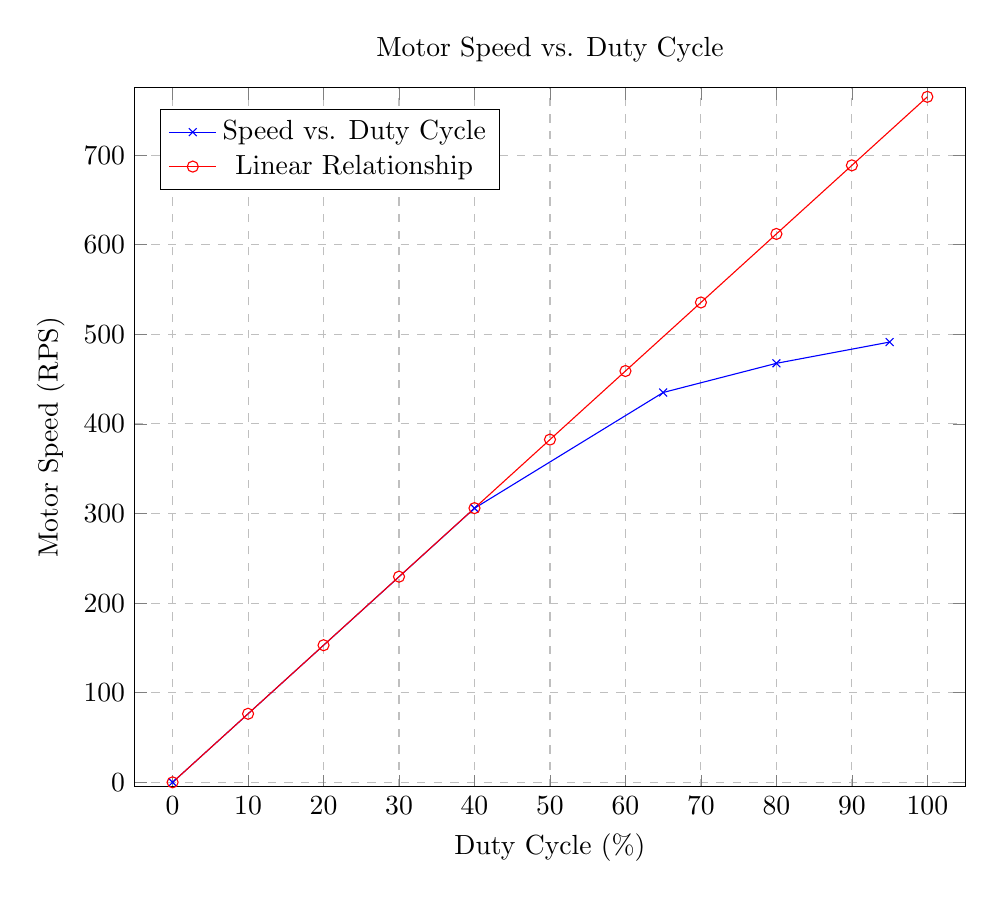
\begin{tikzpicture}
\begin{axis}[
    title={Motor Speed vs. Duty Cycle},
    width=\textwidth,
    xmin=-5, xmax=105,
    xlabel={Duty Cycle (\%)},
    ymin=-5, ymax=775,
    ylabel={Motor Speed (RPS)},
    ymajorgrids=true,
    xmajorgrids=true,
    legend pos=north west,
    grid style=dashed,
	]
	\addplot[
		color=blue,
		mark=x,
		]
		coordinates {
    			(0, 0)(40, 305.85)(65, 435.05)(80, 467.6)(95, 491.32)
		};
		\addlegendentry{Speed vs. Duty Cycle}
	\addplot[
		color=red,
		mark=o,
		]
		coordinates {
    			(0, 0)(10, 76.5)(20, 153)(30, 229.5)(40, 306)(50, 382.5)(60, 459)(70, 535.5)(80, 612)(90, 688.5)(100, 765)
		};
		\addlegendentry{Linear Relationship}
\end{axis}
\end{tikzpicture}
\end{center} 

As the above plot shows, the relationship between motor speed and duty cycle is not exactly linear (although very close). This might be in part due to the limited amounts of data collected, or (more likely) the fact that the motor has internal resistances and friction that prevent it from reaching the higher speeds we'd expect at higher duty cycles (if it were linear).

\section{Conclusion}
The purpose of the lab, to use the input capture peripheral to measure a motor's speed, was certainly accomplished. Although the specific mathematical calculation that converts the different timer measurements to an RPS value is slightly non intuitive (in my opinion), the results are in-line with the physical expectations of the motor.

This type of system shows how easy it would be to implement feedback for controlling the motor speed. Pseudo-code is attached below that demonstrates an example of this system:
\newpage
	\begin{mdframed}[backgroundcolor=code-gray, roundcorner=10pt,
								innerleftmargin=5, innertopmargin=5, innerbottommargin=5]	
	\begin{lstlisting}[language=C, caption=Feedback Pseudo-Code, tabsize=2, label={lst:feedback}]
	func input_capture() {
		delta_time = time_new - time_old
		curr_rps = delta_time * conversion_factor

		if (curr_rps > desired_rps)
			new_pwm = curr_pwm > 1 ? curr_pwm - 1 : 0
		else if (curr_rps < desired_rps)
			new_pwm = curr_pwm < 99 ? curr_pwm + 1 : 100

		set_pwm(new_pwm)
	}
	\end{lstlisting}
	\end{mdframed}
	
The general idea is to take the current reading of the motor's RPS, and depending on if that is above or below a desired speed, adjust the PWM output accordingly.

The limiting factors for measuring a signal's frequency are primarily the timer used for the input capture peripheral. We used timer 3 with a prescale value of 256 and a maximum possible period register. This means that the \textit{fastest} possible frequency we could measure would be:

$$f_{max}=\frac{f_{PB}}{t_{PS}}$$

Which corresponds to a frequency of about 39,062 Hz for our current timer configuration. This would be a signal that only allows a single increment of the timer's period register before triggering an interrupt. On the other hand, the slowest possible signal that could be detected by this system is when the period register reaches \textbf{0xFFFF}, or:

$$f_{min}=\frac{f_{PB}}{t_{PS}}\cdot\frac{1}{65,535}$$

This is approximately 0.596 Hz for the current setup. This is obviously drastically affected by the prescale value used for the associated timer. We are using a very large prescale value which greatly reduces the maximum frequency detectable, but gives a very large range of detectable frequencies.

\begin{figure}[H]
\centering
\includegraphics[width=.8\textwidth]{scope_5.png}
\caption{0\% Duty Cycle Data}
\label{fig:data0}
\end{figure}

\begin{figure}[H]
\centering
\includegraphics[width=.8\textwidth]{scope_6.png}
\caption{40\% Duty Cycle Data}
\label{fig:data40}
\end{figure}

\begin{figure}[H]
\centering
\includegraphics[width=.8\textwidth]{scope_7.png}
\caption{65\% Duty Cycle Data}
\label{fig:data65}
\end{figure}

\begin{figure}[H]
\centering
\includegraphics[width=.8\textwidth]{scope_8.png}
\caption{80\% Duty Cycle Data}
\label{fig:data80}
\end{figure}

\begin{figure}[H]
\centering
\includegraphics[width=.8\textwidth]{scope_9.png}
\caption{95\% Duty Cycle Data}
\label{fig:data95}
\end{figure}

\end{document}